\subsection{Human-Robot Interaction (HRI) Module} HRI module is implemented first to get the raw data from the depth sensor and process it to track the skeletal joint positions in real world coordinates. It is developed in C++ using a core library called Boost and NiTE 2 framework is used for the purpose of skeletal joints tracking. This module is deployed on the general purpose computer that is running inside the robot with necessary libraries and drivers.

Boost is a set of libraries for the C++ programming language that provide support for tasks and structures such as linear algebra, pseudo random number generation, multi threading, image processing, regular expressions, and unit testing. It contains over eighty individual libraries.

HRI module is composed of 3 components which are UDP Server, Gesture and Skeleton tracker. Flowchart \ref{fg:hri:flow} shows the data and control flow of this module where the user is asked to select Gesture or Skeleton tracker, when the program is started. It creates 2 threads depending on the selection: 
\begin{itemize}
	\item UDP Server thread - Asynchronously send data to the client and thread is always running. 
	\item Gesture or Skeleton tracker thread - A loop in the thread polls for a new frame from the depth camera till some key is pressed. If loop is interrupted, then the thread is exited and finally program is closed.
\end{itemize}

Gesture and Skeleton tracker serve the purpose in extracting features from the raw data to implement a hand gesture recognition system. However, Skeleton tracker tracks 15 skeletal points in the human body and that leads to very intensive computation. Due to processing limitations of NAO, we chose to use Gesture tracker as it tracks only hand joints. Following sections describe internal working of HRI module.

\begin{figure}
	[h] \centering 
	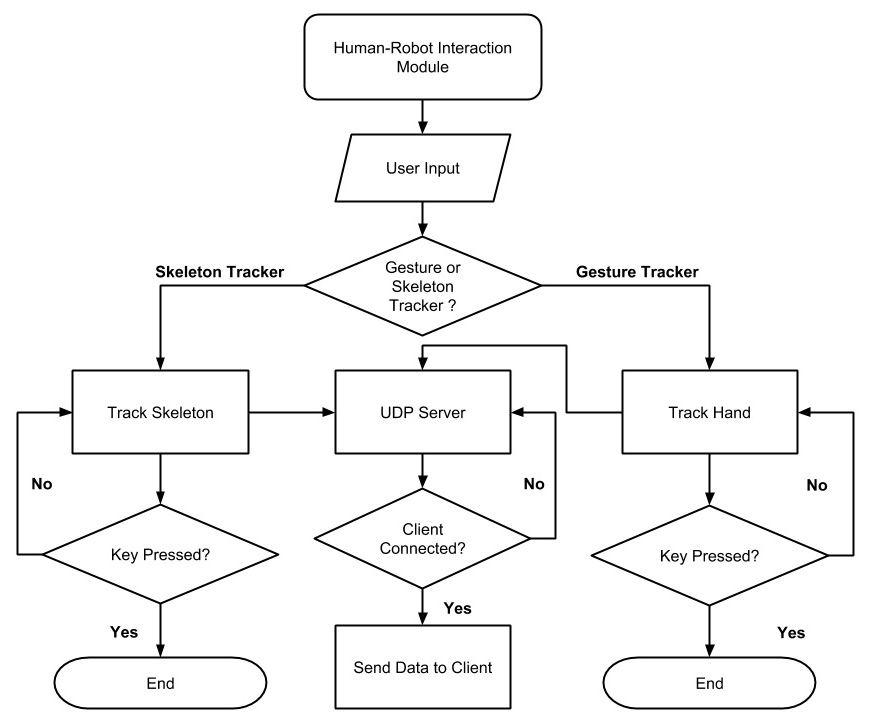
\includegraphics[height=115mm]{figures/content/hri-flow.jpg} \caption{HRI Module Control Flow} \label{fg:hri:flow} 
\end{figure}


\subsubsection{UDP Server} HRI module has to process the raw information from the depth camera and it has to send it to Brain module for the purpose of gesture recognition. As show in the architecture diagram \ref{fg:hri:architecture}, Brain module must be connected via Wireless Local Area Network (WLAN). WLAN at 2.4GHz readily is available on NAO and lead us to a solution, where we have to choose an UDP protocol to transmit the processed data from depth camera. UDP was chosen over other protocols because depth camera produces 30 depth images per second and transferring such a large amount of data using conventional communication technologies such as TCP will be create much overhead and delay in the communication.

Due to asynchronous requirement of the server, Boost Asio library is used to implement UDP server. Boost.Asio is a cross-platform C++ library for network and low-level I/O programming that provides developers with a consistent asynchronous model using a modern C++ approach.

UDP Server is basically an asynchronous programs that creates an UDP socket and listens to an port on the local machine. In this case, we have created a common configuration file named as \textit{hri.json} that contains port numbers for each module in this project. Therefore, this server listens to the 5005 on NAO and waiting for the clients to connect. 

Once the client is connected, it stores the endpoint details of the client such as IP address and the port number of the UDP client (Brain module), so that it can communicate with the Brain module whenever there is some data to be transmitted. Asynchronous functionality Boost.Asio calls the callback handler only when there is communication with the clients and waits in the thread for the next communication.

\subsubsection{Gesture Tracker} \label{sec:hri:ges} Gesture tracker is a component of HRI module that makes use of NiTE framework to localize the hand of the user in the field of view and track the hand position till the hand leaves the field of view (FOV) or hand is touching another object or hidden by an object. 

It uses \textit{HandTracker} class of NiTE framework and it needs to go through following steps before it can track a hand. Section \ref{sec:nite} discusses extensively about the functionalities of NiTE framework.
\begin{itemize}
	\item NiTE framework must be initialized using \textit{nite::initialize()} function. 
	\item Depth camera must be connected and \textit{nite::HandTracker} must be created using OpenNI compatible device id. If not, default depth camera will be selected. 
	\item NiTE focus gesture WAVE must be initiated to localize the hand at first. 
	\item \textit{nite::HandTrackerFrameRef} must be read continuously for a new gesture. 
	\item If WAVE gesture is detected, then hand tracking will be started using the position of hand that triggered the gesture. 
\end{itemize}

Once the hand is been tracked, the hand will be added an id and it will be added to \textit{HandTrackerFrameRef}. NiTE framework allow users to add many number of hands and it will be tracked till there is enough computation power and hands are not overlapping. \textit{HandTrackerFrameRef} contains the array of all active hands and every hand is an object of \textit{nite::HandData}. It contains the position of the hand in 3 dimensional float stored in a class called \textit{Point3f}.

Unlike \textit{nite::UserTracker}, \textit{HandTracker} class can return only the hand position in the space and it can not specify whether it is a left or right hand. It is very necessary information for hand gesture training and classification because confused hand names will lead to a false model of the hand gesture and ultimately resulting in a bad performance. Hence, we have implemented a simple logic with the help of an assumption that user will gesticulate the focus gesture only in the order of right hand first and left hand second. 

Four integer variables \textit{leftHand}, \textit{rightHand}, \textit{lastLostHand} and \textit{handsSize} are used to find whether tracked hand is left or right. The logic behind is that when \textit{handsSize} and \textit{lastLostHand} is zero and a new hand is found, that is considered as right hand and its \textit{nite::HandData::HandId} is stored in the variable \textit{rightHand}. Respectively, the next hand is stored as \textit{leftHand} and \textit{handsSize} counter is increased. If a hand is lost or not tracking, then \textit{lastLostHand} will be updated with the id of the hand that was lost. When there is a new hand and \textit{handsSize} and \textit{lastLostHand} are not zero, then new \textit{handId} will be set to \textit{leftHand} or \textit{rightHand} based on \textit{lastLostHand} variable.

However, functionalities gesture tracker are not only to track hand, but also send these information to Brain module via UDP. Therefore, C++ \textit{nite::HandData} objects must be serialized before transmitted over the network. Therefore, we chose JSON serialization and send them across the network as strings as shown in \ref{code:hand:data}
\begin{lstlisting}
	{ "RIGHT": ["275.456", "339.026", "1841.850"], "LEFT": ["-456.289", "353.880", "1761.360"] } 
\end{lstlisting}
\label{code:hand:data}

Furthermore, HRI module send informations such as detected focus gesture and info messages to Brain module as shown in \ref{code:hand:info} to be displayed on the control center dashboard. Info messages helps us to know the status of the hand tracking algorithm which is the core component of HRI module. 
\begin{lstlisting}
	{"GESTURE":"WAVE"} {"GESTURE":"CLICK"} {"INFO": "Found new hand with id 1"} {"INFO": "LEFT Hand is lost"} {"INFO": "RIGHT Hand is lost"} {"INFO": "Both hands are lost"} {"INFO": "LEFT Hand is at FOV"} 
\end{lstlisting}
\label{code:hand:info}

\subsubsection{Skeleton Tracker} Skeleton Tracker is a component of HRI module that is more complex and computational intensive, since it uses \textit{nite::UserTracker} to track 15 bone joints of human body. Like Gesture Tracker in the section \ref{sec:hri:ges}, this component has to follow few procedure before tracking and it starts with an UDP server to unicast joint positions to Brain module.
\begin{itemize}
	\item NiTE framework must be initialized using \textit{nite::initialize()} function. 
	\item Depth camera must be connected and \textit{nite::UserTracker} must be created using OpenNI compatible device id. If not, default depth camera will be selected. 
	\item Pose in front the camera as shown in the figure \ref{fg:ni:skeleton} to let the algorithm calibrate the body position. 
	\item \textit{nite::UserTrackerFrameRef }must be read continuously for a new user and if a new user is found, skeleton tracking will be started. 
\end{itemize}

\begin{figure}
	[h] \centering 
	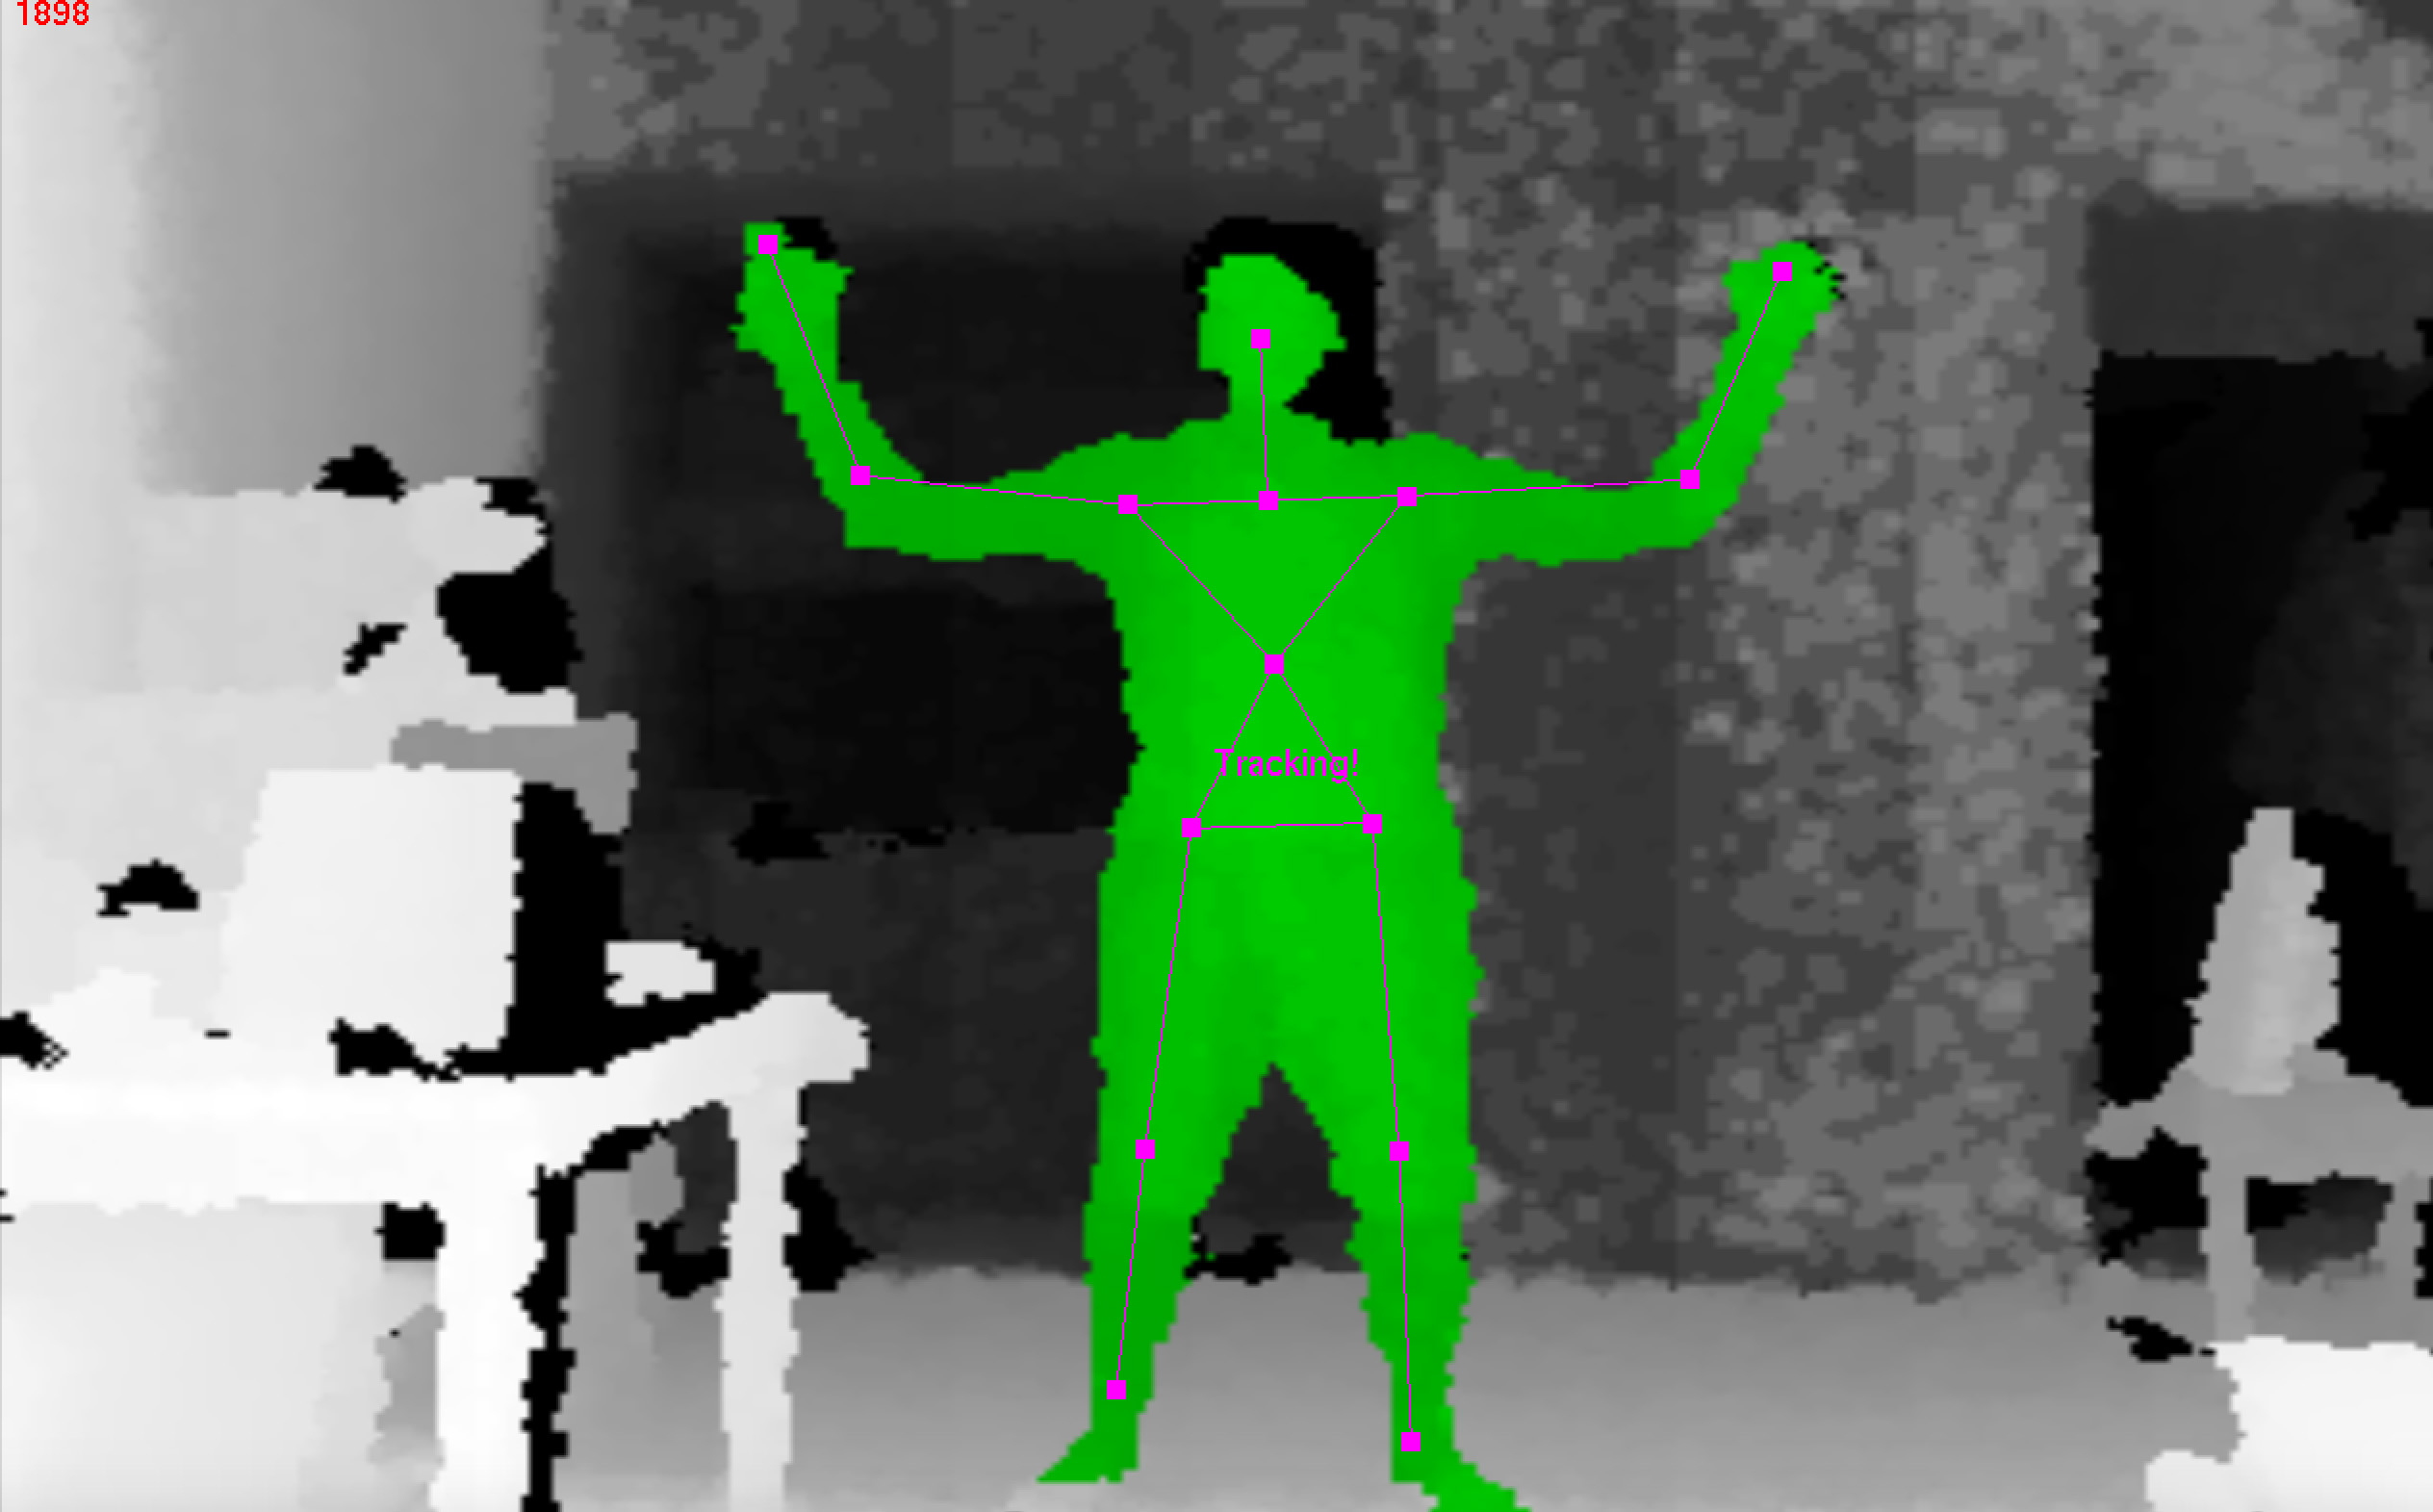
\includegraphics[width=145mm]{figures/content/ni-skeleton.jpg} \caption{Image captured while NiTE tracks 15 skeletal joints of the user using depth camera Asus Xtion. } \label{fg:ni:skeleton} 
\end{figure}


Unlike \textit{nite::HandTracker}, \textit{UserTracker} class of NiTE uses complex algorithms to keep tracking the skeleton even when the user poses in many ways. Therefore, it needs the data provided by NiTE framework which contain models of 1 million training samples. In addition, \textit{UserTracker} can return 15 skeletal joints position and orientation and they are labeled by the joint name. This feature helps us to avoid the implementation to find the hand name. Moreover, details of joint orientations offer us a chance to calculate positions not only in Cartesian coordinates, but also in spherical coordinates system which is essential for many complex hand gesture recognition solutions \cite{21}. Furthermore, \textit{SkeletonJoint} class indicates how sure the NiTE skeleton algorithm is about the joint position. The value is between 0 and 1, with increasing value indicating increasing confidence. Section \ref{sec:nite} discusses extensively about the algorithm of NiTE.

Finally, Skeleton tracker serializes the C++ \textit{nite::UserData} objects to JSON in strings as shown in \ref{code:skeleton:data} in order to asynchronously transfer to the client for further gesture recognition procedures.
\begin{lstlisting}
	{ "HEAD": ["-274.5578", "583.2249", "1933.924"], "NECK": ["-286.0945", "471.8282", "1996.656"], "LEFT_SHOULDER": ["-399.2939", "453.2498", "1975.477"], "RIGHT_SHOULDER": ["-172.895", "490.4066", "2017.835"], "LEFT_ELBOW": ["-673.5372", "389.9277", "1973.389"], "RIGHT_ELBOW": ["77.3149", "437.1607", "2201.007"], "LEFT_HAND": ["-950.7228", "362.1895", "1930.967"], "RIGHT_HAND": ["351.137", "509.7826", "2453.827"], "TORSO": ["-258.3584", "272.1229", "2023.593"], "LEFT_HIP": ["-321.3845", "57.52153", "2033.549"], "RIGHT_HIP": ["-139.8603", "87.31343", "2067.511"], "LEFT_KNEE": ["-313.5818", "-344.5291", "2039.209"], "RIGHT_KNEE": ["-129.7786", "-280.5863", "2110.95"], "LEFT_FOOT": ["-341.4384", "-665.9058", "2189.055"], "RIGHT_FOOT": ["-172.1151", "-559.3973", "2262.547"] } 
\end{lstlisting}
\label{code:skeleton:data}
